\documentclass{article}
\usepackage{amsmath}
\usepackage{amssymb}
\usepackage{algpseudocode}
\usepackage{algorithm}
\usepackage{graphicx}
\usepackage{caption}
\usepackage{subcaption}
\usepackage{float}


\begin{document}
\title{Homework 1 - CMSC-25400}
\author{Patrick Collins}
\date{\today}
\maketitle

\section{Proofs}
\begin{enumerate}
\item Derive an algorithm that can learn any monotone conjunction over
  ${0, 1}^n$ with a mistake bound of $n$. \\

\begin{algorithm}
\caption{Addition for Monotone Conjunctions}
\begin{algorithmic}[1]
\State $f \gets \bigwedge\limits_{n=1}^n x_n$
\State $i \gets 1$
\While{True}
\State predict $\hat{y}^t = f(x^t)$
\If{$(\hat{y}^t == 1)$ and $(y^t == 0)$}
\State remove $\{x | x \in x^t$ if $x == 1$\} from $f$.
\EndIf
\State $t \gets t + 1$
\EndWhile
\end{algorithmic}
\end{algorithm}

Proof of mistake bound:

Note that (a) this algorithm will only ever produce false
negatives, and (b) it removes at least one term from the
concept for every false negative. Therefore, because there are only
$n$ terms total, it can make a maximum of $n$ mistakes. $\blacksquare$

\item Prove that, for any concept class $C$ and online algorithm $A$
  with finite mistake bound $M$, there is a conservative algorithm
  $A'$ with mistake bound $M$ on $C$. 


Claim: Let $A'$ be an algorithm that simulates the action of $A$ on the input
sequence $S$, which changes its hypothesis to the hypothesis currently
held by $A$ only when it makes a mistake. When such a mistake occurs,
let $A'$ remove every $f$ that is inconsistent with the mistake from
the concept class it is currently considering, $C(A')$. Then $M(A') \leq
M(A)$, i.e. the mistake bound of $A'$ is bounded from above by the mistake bound of $A$. 

Lemma 1: After any sequence of inputs, $C(A)$ contains at least as many
incorrect hypotheses as $C(A')$, and both contain the true hypothesis.

Proof: Suppose, for contradiction, that there exists some hypothesis
$f \in C(A), f \not\in C(A')$. Then either $f$ is consistent with the
input that both algorithms have processed so far, or it is not. If it
is not consistent, then $C(A)$ has more incorrect hypotheses than
$C(A')$, which is what we wanted to show. If $f$ is consistent with
the input processed so far, then $A'$ would have never removed it from
$C(A')$, a contradiction.

Alternatively, suppose, for contradiction, that there is some $f
\not\in C(A), f \in C(A')$. $A'$ removes inconsistent hypotheses from
its concept class, so $f$ must be consistent with the input seen so
far. But then $f$ could be the correct hypothesis, and if $A$ had
removed the correct hypothesis from its concept class, then it would
make infinitely many mistakes, a contradiction.

Proof of main claim: The mistakes that any algorithm makes is bounded from
above by the number of incorrect hypotheses in the concept class its
considering, so, the fact that $C(A') \leq C(A)$ over any sequence of
inputs by lemma 1 implies that $M(A') \leq M(A)$ for any sequence of
inputs, which is what we wanted to show. Hence $A'$ has a mistake
bound of $M$ over $C$. $\blacksquare$

\item Prove that $cost_{IC} = 2cost_{avg^2}$

Beginning with the simple case of a single cluster center:

\begin{align*}
  cost_{IC}(C) &= \frac 1 {|C|} \sum\limits_{x} \sum\limits_{x'} (x - x')^2\\
  &= \frac 1 {|C|} \sum\limits_{x} \sum\limits_{x'} ||x - x'||\\
  &= \frac 1 {|C|} \sum\limits_{x} \sum\limits_{x'} (x^T - x'^T)(x - x')\\
  &= \frac 1 {|C|} \sum\limits_{x} \sum\limits_{x'} (x^Tx - x^Tx' - x'^Tx + x'^Tx')\\
  &= \frac 1 {|C|} \sum\limits_{x} \sum\limits_{x'} x^Tx -  \frac 1 {|C|} \sum\limits_{x} \sum\limits_{x'} x^Tx' -  \frac 1 {|C|} \sum\limits_{x} \sum\limits_{x'}x'^Tx +  \frac 1 {|C|} \sum\limits_{x} \sum\limits_{x'} x'^Tx'
\end{align*}
Noting that:
\begin{align*}
  \sum\limits_{x} \sum\limits_{x'} x^Tx &= |C| \sum\limits_{x} x^Tx\\
  \sum\limits_{x} \sum\limits_{x'} x'^Tx' &= |C| \sum\limits_{x'} x'^Tx'\\
  \sum\limits_{x'} x'^Tx' &= \sum\limits_{x} x^Tx\\
\end{align*}

and 

\begin{align*}
  \sum\limits_{x} \sum\limits_{x'} x^Tx' = \sum\limits_{x} \sum\limits_{x'} x'^Tx
\end{align*}


We can collect like terms:

\begin{align*}
  \frac 1 {|C|} \sum\limits_{x} \sum\limits_{x'} (x^Tx - x^Tx' - x'^Tx + x'^Tx') &= 2\sum\limits_x x^Tx - \frac 2 {|C|} \sum\limits_{x} \sum\limits_{x'} x^Tx'\\
   &= 2(\sum\limits_x x^Tx - \frac 1 {|C|} \sum\limits_{x} x^T \sum\limits_{x} x)
 \end{align*}
 
Then, we begin to work from the other side of the equation. Noting
that 
\begin{align*}
  m = \frac {\sum\limits_{x'} x'} {|C|}
\end{align*}

We have:

\begin{align*}
  cost_{avg^2}(C) &= \sum\limits_{x} d(x, \frac {\sum\limits_{x'} x'} {|C|})^2\\
  &= \sum\limits_{x} ||x - \frac {\sum\limits_{x'} x'} {|C|}||^2\\
  &= \sum\limits_{x} (x - \frac {\sum\limits_{x'} x'} {|C|})^T (x - \frac {\sum\limits_{x'} x'} {|C|})\\
    &= \sum\limits_{x} (x^Tx - x^T \frac {\sum\limits_{x'} x'} {|C|} - \frac {\sum\limits_{x'} x'} {|C|}^Tx + \frac {\sum\limits_{x'} x'} {|C|}^T \frac {\sum\limits_{x'} x'} {|C|})\\
    &= \sum\limits_{x} x^Tx - \frac 1 {|C|} \sum\limits_{x} x^T \sum\limits_{x'} x' -  \frac 1 {|C|}  \sum\limits_{x'} x'^T \sum\limits_{x} x +  \frac 1 {|C|^2} \sum\limits_{x} x (\sum\limits_{x'} x'^T \sum\limits_{x'} x')\\
   &= \sum\limits_{x} x^Tx - \frac 2 {|C|} \sum\limits_{x} x^T \sum\limits_{x'} x' +  \frac 1 {|C|} \sum\limits_{x'} x'^T \sum\limits_{x'} x'\\
   &= \sum\limits_{x} x^Tx - \frac 1 {|C|} \sum\limits_{x} x^T \sum\limits_{x} x 
\end{align*}

Noting that the both the
intra-cluster distance and the $k$-means cost within a single cluster
do not depend on how many other clusters there are, we can simply add
back in the summation on $k$, and get:

\begin{align*}
  cost_{IC}(C_0 \cup C_1,\dots,\cup C_k) &= \sum\limits_i^k 2(\sum\limits_{x \in C_i} x^Tx - \frac 1 {|C_i|} \sum\limits_{x \in C_i} x^T \sum\limits_{x \in C_i} x)\\
  &= 2\sum\limits_i^k(\sum\limits_{x \in C_i} x^Tx - \frac 1 {|C_i|} \sum\limits_{x \in C_i} x^T \sum\limits_{x \in C_i} x)\\
  cost_{avg^2}(C_0 \cup C_1,\dots,\cup C_k) &= \sum\limits_i^k(\sum\limits_{x} x^Tx - \frac 1 {|{x \in C_i}|} \sum\limits_{x} x^T \sum\limits_{x} x)
\end{align*}

$\blacksquare$

\item Results from applying KMeans:

\begin{figure}[H]
  
\includegraphics{../output/small.png}
\end{figure}
\begin{figure}[H]
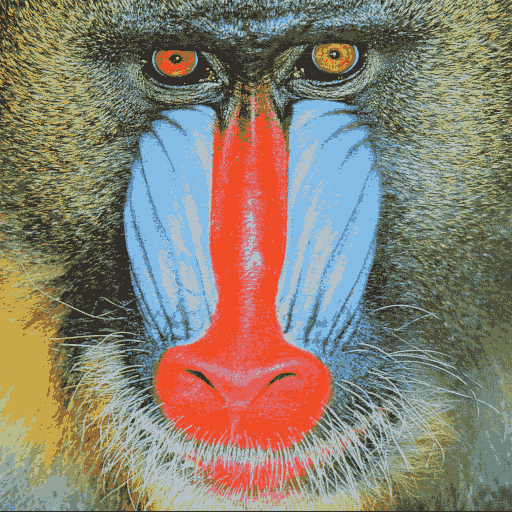
\includegraphics{../output/large.png}
\end{figure}

\pagebreak
The contrast in the resulting, compressed image is higher, reflecting
the fact that the number of colors in the pictures has been halved. It
also appears to be somewhat more washed-out than the original.

This compression reduces the total number of colors to 16, meaning
that each pixel can be represented with three 4-bit numbers rather
than 8-bit ones, resulting in a compression ratio of approximately
50\% for large images, because the storage requirement for each pixel
has been halved. 




\end{enumerate}
\end{document}
